\subsection{Segment lungs in XRay(s)}
\label{sec:warmup5}

    Lung segmentation from X-rays are required to automate boundary detection, enhancing diagnostic accuracy and efficiency in medical imaging analysis. In this exercise, we were given chest X-ray images of patients, and the segmented masks of their lungs. We need to employ a deep learning model that can segment lungs from XRays or find boundaries of the lungs.

\subsubsection{Dataset}

    The provided dataset have $50$ training x-ray images and $10$ testing images, with their corresponding masks, thus we can observe that the provided dataset is very small. As there was no validtion set, I have randomly splited the training dataset into validation and training set in ration 1:9 respictively. The images in this dataset were converted to grayscale images with shape $256 \times 256$.

\subsubsection{Training}

    This being a segmentation problem, an encoder-decoder type of model needs to be employed. I have created a UNet as shown in \cref{fig:unet_lung}. The model have a resnet18 encoder block which was pretrained on imagenet1k dataset and a decoder block. As the model might suffers from gradient vanishing, skip connections is used, thus a UNet is structure is achieved. Since, I am predicting the pixels of an image as $0$ or $1$, binary cross-entropy error was used for training with Adam optimizer with learning rate of $10^{-3}$. \Cref{fig:lung-segmentation-learning-curve} illustrates the learning curve of the training and validation sets.

    \begin{figure}[htbp]
        \centering
        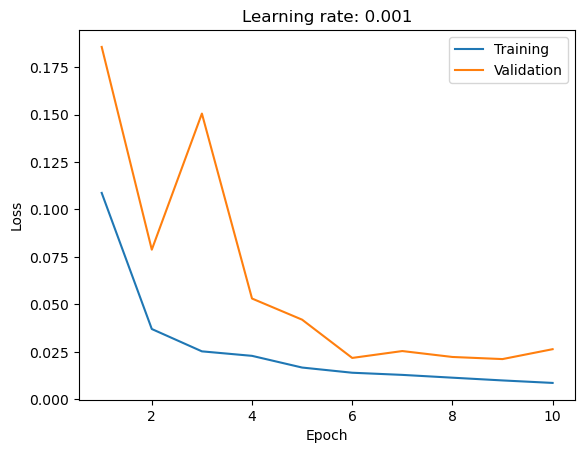
\includegraphics[width=\linewidth]{../plots/segmentation/learning.png}
        \caption{Lungs segmentation model learning curve on training and validation sets}
        \label{fig:lung-segmentation-learning-curve}
    \end{figure}

\subsubsection{Results}

    From the learning curve in \cref{fig:lung-segmentation-learning-curve} we can observe that the model have converged to lowest loss, and is not overfited on the dataset. The trained model is then tested on test set, and got mIoU score of $0.933$ and mDICE score of $0.965$. \Cref{fig:lung-segmentation-result} shows the predicted lung mask of a XRay and we can observe that model is able to generate masks which is similar to ground truth mask.

    \begin{figure}[htbp]
        \centering
        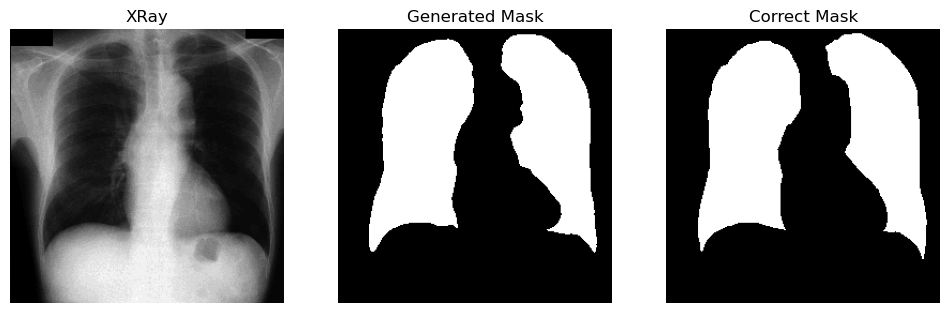
\includegraphics[width=\linewidth]{../plots/segmentation/result.png}
        \caption{Predicted lung mask of an XRay by trained UNet}
        \label{fig:lung-segmentation-result}
    \end{figure}